%\documentstyle[times,art10,twocolumn,latex8]{article}

\documentclass[times, 10pt,twocolumn]{article} 
\usepackage{latex8}
\usepackage{times}

\usepackage{graphicx,times,amsmath} % Add all your packages here
\usepackage{amsfonts}
%\usepackage{listings}

\usepackage[cp1250]{inputenc}  % or [cp1250], or [latin2], or whatever
                               % suitable for your system


\usepackage{url}

\pagestyle{empty}

% correct bad hyphenation here
\hyphenation{op-tical net-works semi-conduc-tor IEEEtran}

\begin{document}

\title{Fuzzy Classification of Web Reports with Linguistic Text Mining}

\author{Jan Dedek\\
Department of Software Engineering\\
Charles University in Prague, Czech Republic\\
email: jan.dedek@mff.cuni.cz
\and
Peter Vojtas\\
Department of Software Engineering\\
Charles University in Prague, Czech Republic\\
peter.vojtas@mff.cuni.cz\\
}


\maketitle              % typesets the title of the contribution
\thispagestyle{empty}



\begin{abstract}
In this paper we present a fuzzy system which provides a fuzzy classification of textual web reports. Our approach is based on usage of third party linguistic analyzers, our previous work on web information extraction and fuzzy inductive logic programming. Main contributions are formal models and prototype implementation of the system and evaluation experiments. 
\end{abstract}

% no key words

\section{Introduction}

%Big amount of information on the web increases the need of automated precessing. Especially textual information are hard for machine processing and understanding. Crisp methods have their limitations. In this paper we present a fuzzy system which provides a fuzzy classification of textual web reports. 


Our motivating example are messages of accident reports on the web. We would like to have a tool which is able to classify such message with degree of being it a serious accident. 

Our solution is based first on information extraction (see  emphasized information to be extracted) and second on processing this information to get fuzzy classification rules. In this paper we are concentrated on the second phase -- a fuzzy classification.

%\begin{figure}[hb!]
%\centerline{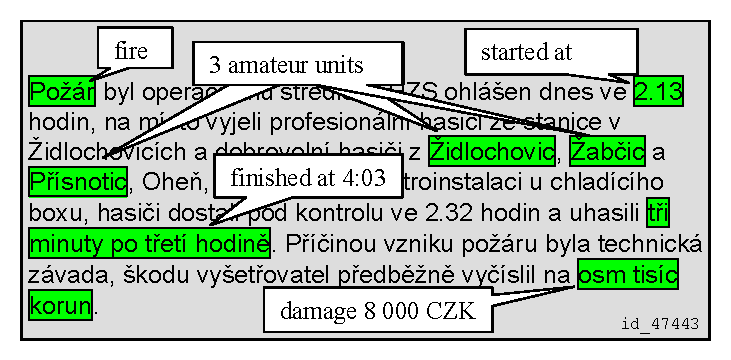
\includegraphics[width=\hsize]{img/message}}
%\caption{Example of analyzed web report.}
%\label{img:message}
%\end{figure}

Main contributions of this paper can be stated as follows: 
\\$\bullet$ formal models for fuzzy classification of information form web reports
\\$\bullet$ prototype implementation of a fuzzy classification system
\\$\bullet$ experimental evaluation of the fuzzy classification system



%\subsection{Related work}
%There is a plenty of systems dealing with text mining and text classification, let us mention at least some. In \cite{biblio:ReYaLiOntoText08} authors use ontology modeling to enhance text identification. In \cite{biblio:CAP} authors use preprocessed data from National Automotive Sampling System and test various soft computing methods to modeling severity of injuries (some hybrid methods showed best performance). Methods of Information Retrieval (IR) are very numerous, with extraction mainly based on key word search and similarities. Connecting IR and text mining techniques with web information retrieval can be found in Chapter Opinion mining in the book of Bing Liu \cite{biblio:WebDataMining}. 
%
%Our paper is organized as follows: In Chapter 2 we develop our models and methods and design the system, focusing on description of the linguistic analyzer, ILP, fuzzy ILP and several translations of fuzzy ILP to crisp ILP. In Chapter 3 we describe the system prototype and settings of our experiments, especially data preparation. In Chapter 4 we describe results of our experiments and provide comparison of used methods. 


%%%%%%%%%%%%%%%%%%%%%%%%%%%%%%%%%%%%%%%%%%%%%%%%%%%%%%%%%%%%%%%%%%%%%%%%%%%%%%%%%%%%%%%%%%%%%%%%%
\section{Models, methods, design of the system}
%%%%%%%%%%%%%%%%%%%%%%%%%%%%%%%%%%%%%%%%%%%%%%%%%%%%%%%%%%%%%%%%%%%%%%%%%%%%%%%%%%%%%%%%%%%%%%%%%

General schema of our system is in Fig~\ref{img:schema}. We use our previously developed web information extraction tools based on third party linguistic analyzer (the upper two dashed arrows). The classification is based on fuzzy ILP and its translation to several crisp ILP tasks. We assume that a small amount of learning data are annotated by a human.

\begin{figure}[hb!]
\centerline{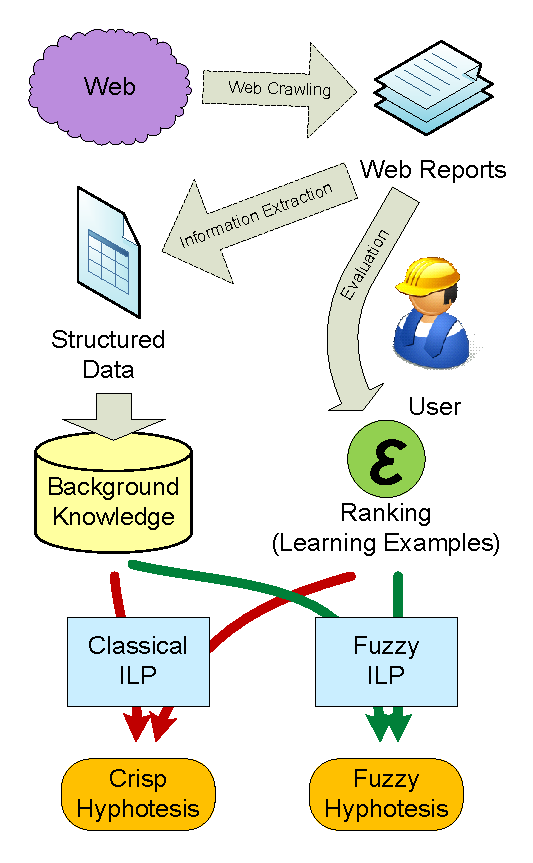
\includegraphics[width=.7\hsize,height=\hsize]{img/schema}}
\caption{Schema of the whole system.}
\label{img:schema}
\end{figure}

%\subsection{Linguistic Analyzer}
%In this section we will briefly describe the linguistic tools that
%we have used to produce linguistic annotation of texts. 
%These tools are being developed in the Institute of Formal
%and Applied Linguistics in Prague, Czech Republic. They
%are publicly available � they have been published on a CDROM
%under the title PDT 2.0 \cite{biblio:PDT20_CD} (first five tools) and in
%\cite{biblio:KlTransformationBasedTectogrammatical2006} (Tectogrammatical analysis). These tools are used as a
%processing chain and at the end of the chain they produce
%tectogrammatical \cite{biblio:MiBeAnnotationtectogrammatical2006} dependency trees. 
%
%
%Tool 1. Segmentation and tokenization consists of tokenization
%(dividing the input text into words and punctuation)
%and segmentation (dividing a sequences of tokens
%into sentences).
%
%Tool 2. Morphological analysis assigns all possible lemmas
%and morphological tags to particular word forms (word
%occurrences) in the text.
%
%Tool 3. Morphological tagging consists in selecting a single
%pair lemma-tag from all possible alternatives assigned
%by the morphological analyzer.
%
%Tool 4. Collins� parser � Czech adaptation. 
%Unlike the usual approaches to the description of
%English syntax, the Czech syntactic descriptions are
%dependency-based, which means, that every edge of
%a syntactic tree captures the relation of dependency
%between a governor and its dependent node. Collins�
%parser gives the most probable parse of a given input
%sentence.
%
%Tool 5. Analytical function assignment assigns a description
%(analytical function � in linguistic sense) to every edge
%in the syntactic (dependency) tree.
%
%Tool 6. Tectogrammatical analysis produces linguistic annotation
%at the tectogrammatical level, sometimes called
%�layer of deep syntax�. Such a tree can be seen on
%the See Fig~\ref{img:tree}. Annotation of a sentence at this layer
%is closer to meaning of the sentence than its syntactic
%annotation and thus information captured at the tectogrammatical
%layer is crucial for machine understanding
%of a natural language \cite{biblio:KlTransformationBasedTectogrammatical2006}.

%\subsection{Web Information Extraction}

%Having Web resource content analyzed by above linguistic tools, we have data stored in the form of tectogramatic trees. To achieve our objectives we have to extract information from this representation. 
Here we refer to our previous work %\cite{biblio:DeVoLinguisticextraction2008,biblio:DeVoComputingaggregations2008, 
\cite{biblio:DeEcExperimentswith2008}. A long path of tools starting with web crawling and resulting with the extracted structured information is developed in our previous work. 
%In Fig~\ref{img:tree} we can see nodes of tree were information about damage (8000 CZK) is located. We have used Inductive logic Programming to learn rules which are able to detect such nodes. In this paper we will concentrate on the usage of such extracted information to be able to classify content. 
%Let us note, that this extraction process requires some human assistance when annotating data.

%Note that our method is general and is not limited to Czech and can be used with any structured linguistic representation. 


%
%\begin{figure}[hb!]
%\centerline{\framebox{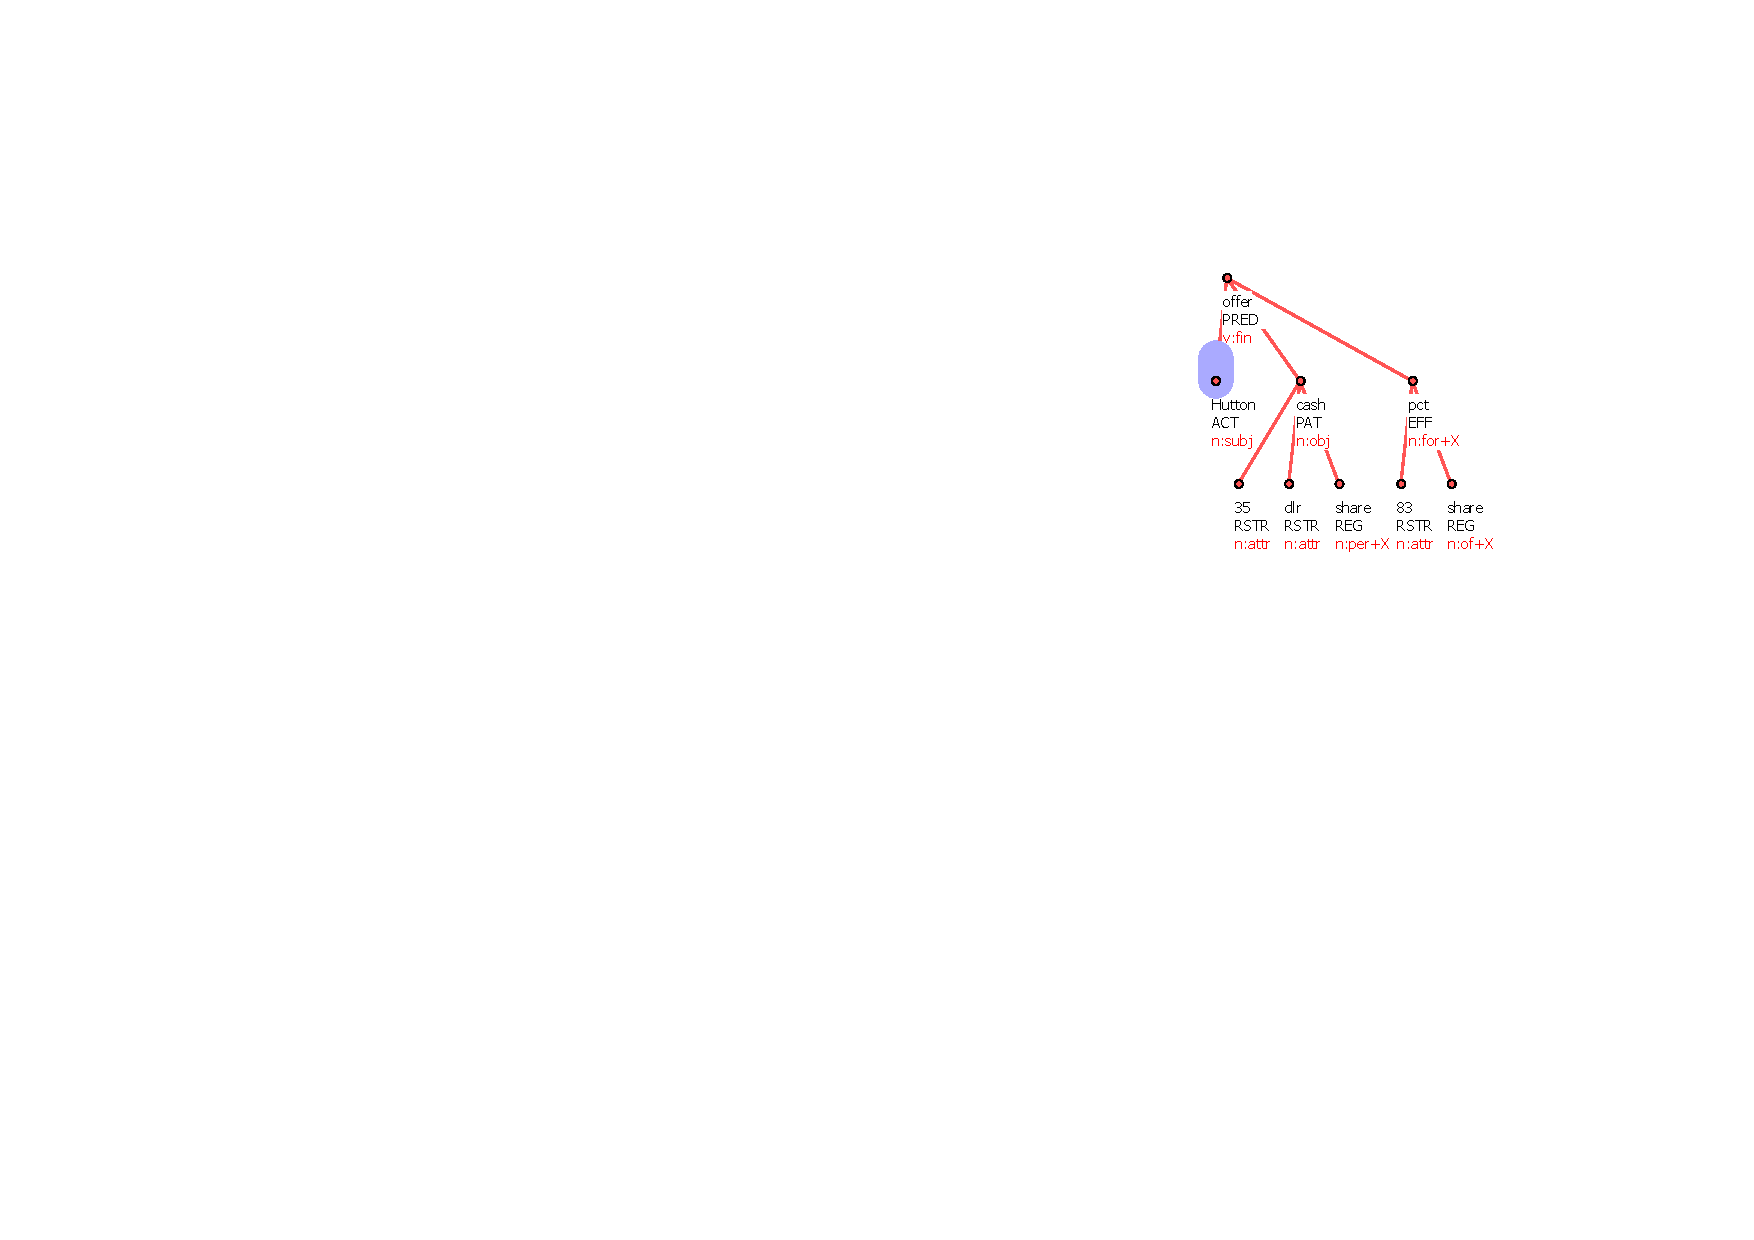
\includegraphics[width=\hsize]{img/tree}}}
%\caption{Example of linguistic tree of one of analyzed sentences.}
%\label{img:tree}
%\end{figure}
%
%



%\subsection{Classical ILP}
%
%In our application we are facing the challenge of induction and/or mining on several places. First we need an inductive procedure when extracting from web texts attributes of an accident. 
%
%Second (the subject of this paper) we need an inductive procedure when trying to explain degree of seriousness of an accident by attributes of this accident (also called background knowledge).

%Both places where induction has to be used have following requirements
%
%
%\begin{itemize}
%	\item data are/can be fuzzy
%	\item background knowledge is multirelational (representation of tectogramatical trees)
%	\item classification is fuzzy
%\end{itemize}
%
%Having in mind these requirements we chose fuzzy inductive logic programming. To make the paper readable we present bellow short description of ILP techniques.

%
%Given is a set of examples $E=P\cup N$, where $P$ contains positive and $N$ negative examples, and a background knowledge $B$. The task is to find a hypothesis $H$ such that 
%
%$$
%(\forall e\in P)(B\cup H\models e)
%$$
%and
%$$
%(\forall e\in N)(B\cup H\not\models e).
%$$
%Typically, $E$ consists of ground instances of the target predicate which has to be classified - in our case accidents. $B$ typically consists of several predicates (relational tables) which describe properties of object which have to be classified - in our case properties of accidents. Background knowledge can contain also some rules. Hypothesis $H$ typically consists of logic programming rules, which when added to $B$, explain all positive examples and no negative examples.

%Main advantage of ILP is it's multirelational character, namely $B$ can reside in several tables.



\subsection{Fuzzy and GAP induction}

In our presentation of Inductive Logic Programming (ILP) we follow \cite{dzeroski2001:relat_dm} and  \cite{biblio:Muggleton94inductivelogic}, for fuzzy Inductive Logic Programming (fILP) we follow the paper of T. Horvath and P. Vojtas \cite{biblio:FILP} about fuzzy inductive logic programming.

We use the approach of the fuzzy logic in narrow sense developed by J. Pavelka \cite{biblio:Pavelka} and P. Hajek \cite{biblio:Hajek}. Formulas are of the form $\varphi, x$ ($\varphi$ is syntactically same as in the crisp case) are graded by a truth value $x\in [0,1]$.
A structure ${\mathcal M}$ consist of domain $M$ and relations are interpreted fuzzy (we do not consider function symbols here). Evaluation $\left\|\varphi\right\|_{{\mathcal M}}$ of a formula $\varphi$ uses truth functions of many valued connectives (our logic is extensional and/or truth functional). Satisfaction is defined by ${\mathcal M}\models_f (\varphi, x)\ iff\ \left\|\varphi\right\|_{{\mathcal M}}\ge x$

Given is a fuzzy set of examples ${\mathcal E}:E\longrightarrow [0,1]$ and a fuzzy background knowledge ${\mathcal B}:B\longrightarrow [0,1]$. The task is to find a fuzzy hypothesis ${\mathcal H}:H\longrightarrow [0,1]$ such that 

$(\forall e,f\in E)(\forall {\mathcal M})({\mathcal M}\models_f {\mathcal B}\cup {\mathcal H})$
we have\\ ${\mathcal E}(e)>{\mathcal E}(f)\Rightarrow \left\|e\right\|_{{\mathcal M}}\ge \left\|f\right\|_{{\mathcal M}}.$ That is, it cannot happen that ${\mathcal E}(e)>{\mathcal E}(f) \wedge \left\|e\right\|_{{\mathcal M}}< \left\|f\right\|_{{\mathcal M}},$ or rephrased, if ${\mathcal E}$ is rating $e$ higher than $f$, then it can not happen in a model of ${\mathcal B}\cup {\mathcal H}$ that $e$ is rated worse than $f$.

Typically, ${\mathcal E}$ consists of ground instances of the target predicate which are  classified in truth degrees - in our case degree of seriousness of an accident. ${\mathcal B}$ typically consists of several fuzzy predicates (fuzzy relational tables) which describe properties of object which have to be classified - in our case fuzzy properties of accidents - degree of injury, degree of damage, .... 
%Background knowledge can contain also some rules, so far only crisp rules are used.
Hypothesis ${\mathcal H}$ typically consists of a fuzzy logic program, which when added to ${\mathcal B}$, prevents of misclassification (better can not be declared to be worse, nevertheless can be declared as having same degree (for more detailed discussion on this definition of fuzzy ILP we refer to the paper \cite{biblio:FILP})). Moreover, in practice, we use GAP - Generalized Annotated Programs, so graded formulas will be sometimes understood as annotated (with crisp connectives and more complex annotation of head of rules). This is possible, because in \cite{biblio:KLV} we have shown that (some extension of) fuzzy logic programming is equivalent to (some restriction of) generalized annotated programs. 

\subsection{Translation of fuzzy ILP task to several classical ILP tasks}

As far as there is no implementation of fuzzy (GAP) ILP, we have to use a classical ILP system. Fortunately a fuzzy ILP task can be translated to several crisp ILP tasks (subject to some rounding and using finite set of truth values).

Assume, our fuzzy sets take values for a finite set of truth values $\{0,1\}\subseteq T\subseteq [0,1]$. For each predicate $p(x)$ in $B$ we add an additional attribute for truth value $p(x,t)$. We construct two crisp background knowledge sets  ${\mathcal B}^{raw}_T$ and ${\mathcal B}^{mon}_T$  as follows:

First is a direct coding of the fuzzy value by an additional attribute:

If ${\mathcal B}(p(x))=t\in T$, then for we add $p(x,t')\in {B}^{raw}_T$.

Second is obtained by a process called monotonization:

If ${\mathcal B}(p(x))=t\in T$, then for all $t'\in T, t'\le t$ we add $p(x,t')\in {B}^{mon}_T$.

Also example sets are constructed in two ways.

For all $t\in T$ we create a crisp example set $E_t=P_t\cup N_t$, where $e\in P_t \ \ iff \ \ {\mathcal E}(e)= t$ and $N_t$ is the rest of $E$.


For all $t\in T$ we create a crisp example set $E_{\ge t}=P_{\ge t}\cup N_{< t}$, where $e\in P_{\ge t} \ \ iff \ \ {\mathcal E}(e)\ge t$ and $N_t$ is the rest of $E$.

These two translation create two ILP tasks, first is purely crisp and second can be understood (and translated back to) fILP.

First \textit{raw ILP task} is for each $t\in T$ given by $E_t$ and $B^{raw}_{T}$, as a result we get a set of hypothesis $H_t$.

Second, for each $t\in T$ we create a crisp ILP task $E_{\ge t}, {B}^{mon}_T$ and get a hypothesis $H_{\ge t}$ guaranteeing examples of degree at least $t$. Note that variable boundings in $B$ have no boundings on truth value attribute, which was added to each predicate, and hence there are no variable boundings in $H_{\ge t}$ on truth value attribute. To predicates in $E$ we did not add the additional truth value attribute

Now we sketch the translation of second ILP task to GAP (fILP) rules. Let us assume $C$ is the target predicate in the domain of ${\mathcal E}$. We define ${\mathcal H}$ with domain consisting of one GAP rule $C(y):u(x_1,\dots,x_m)\leftarrow B_1:x_1 \&\dots\& B_n:x_m,$
here $B_1:x_1 \&\dots\& B_n:x_m$ is enumeration of all predicates in $B$.

Assume $B_1(y_1,t_1),\dots,B_n(y_n,t_n)$ are some predicates in $B$ (for simplicity enumerated from 1 to $n\le m$). Then for each rule $R=C(y)\Leftarrow B_1(y_1,t_1),\dots,B_n(y_n,t_n)$ in $H_t$ we give a constraint in definition of $u$ as follows
$$
U_R=u(x_1,\dots,x_m)\ge t \hbox{ if }x_1\ge t_1,\dots,x_n\ge t_n.
$$
Note that $x_{n+1},\dots,x_m$ have no restrictions.

We claim, that if all $H_t$ were correctly learned by an crisp ILP system then for $u$ the minimal solution of all constraints $U_R$ for all $R\in H_t$, for all $t\in T$, the rule
$$
C(y):u(x_1,\dots,x_m)\leftarrow B_1:x_1 \&\dots\& B_n:x_m,
$$
is a correct solution to fuzzy ILP task given by ${\mathcal E}$ and ${\mathcal B}$. Our presentation is here a little bit simplified and we freely switch between fuzzy and GAP programs, which are know to be equivalent, see  \cite{biblio:KLV}.


\begin{figure}
\centerline{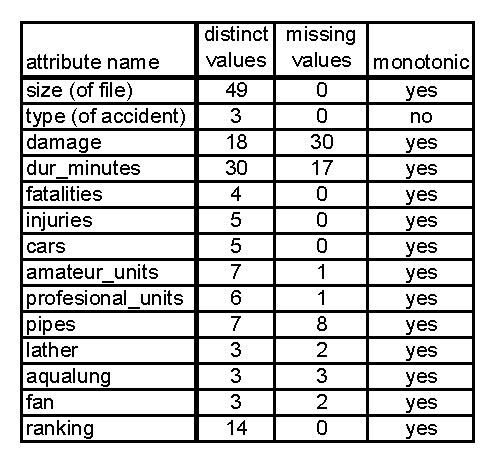
\includegraphics[width=.7\hsize]{img/attributes_description}}
\caption{Accident attributes.}
\label{img:attributes_description}
\end{figure}

\begin{figure}[b!]
Crisp learning examples\\
\centerline{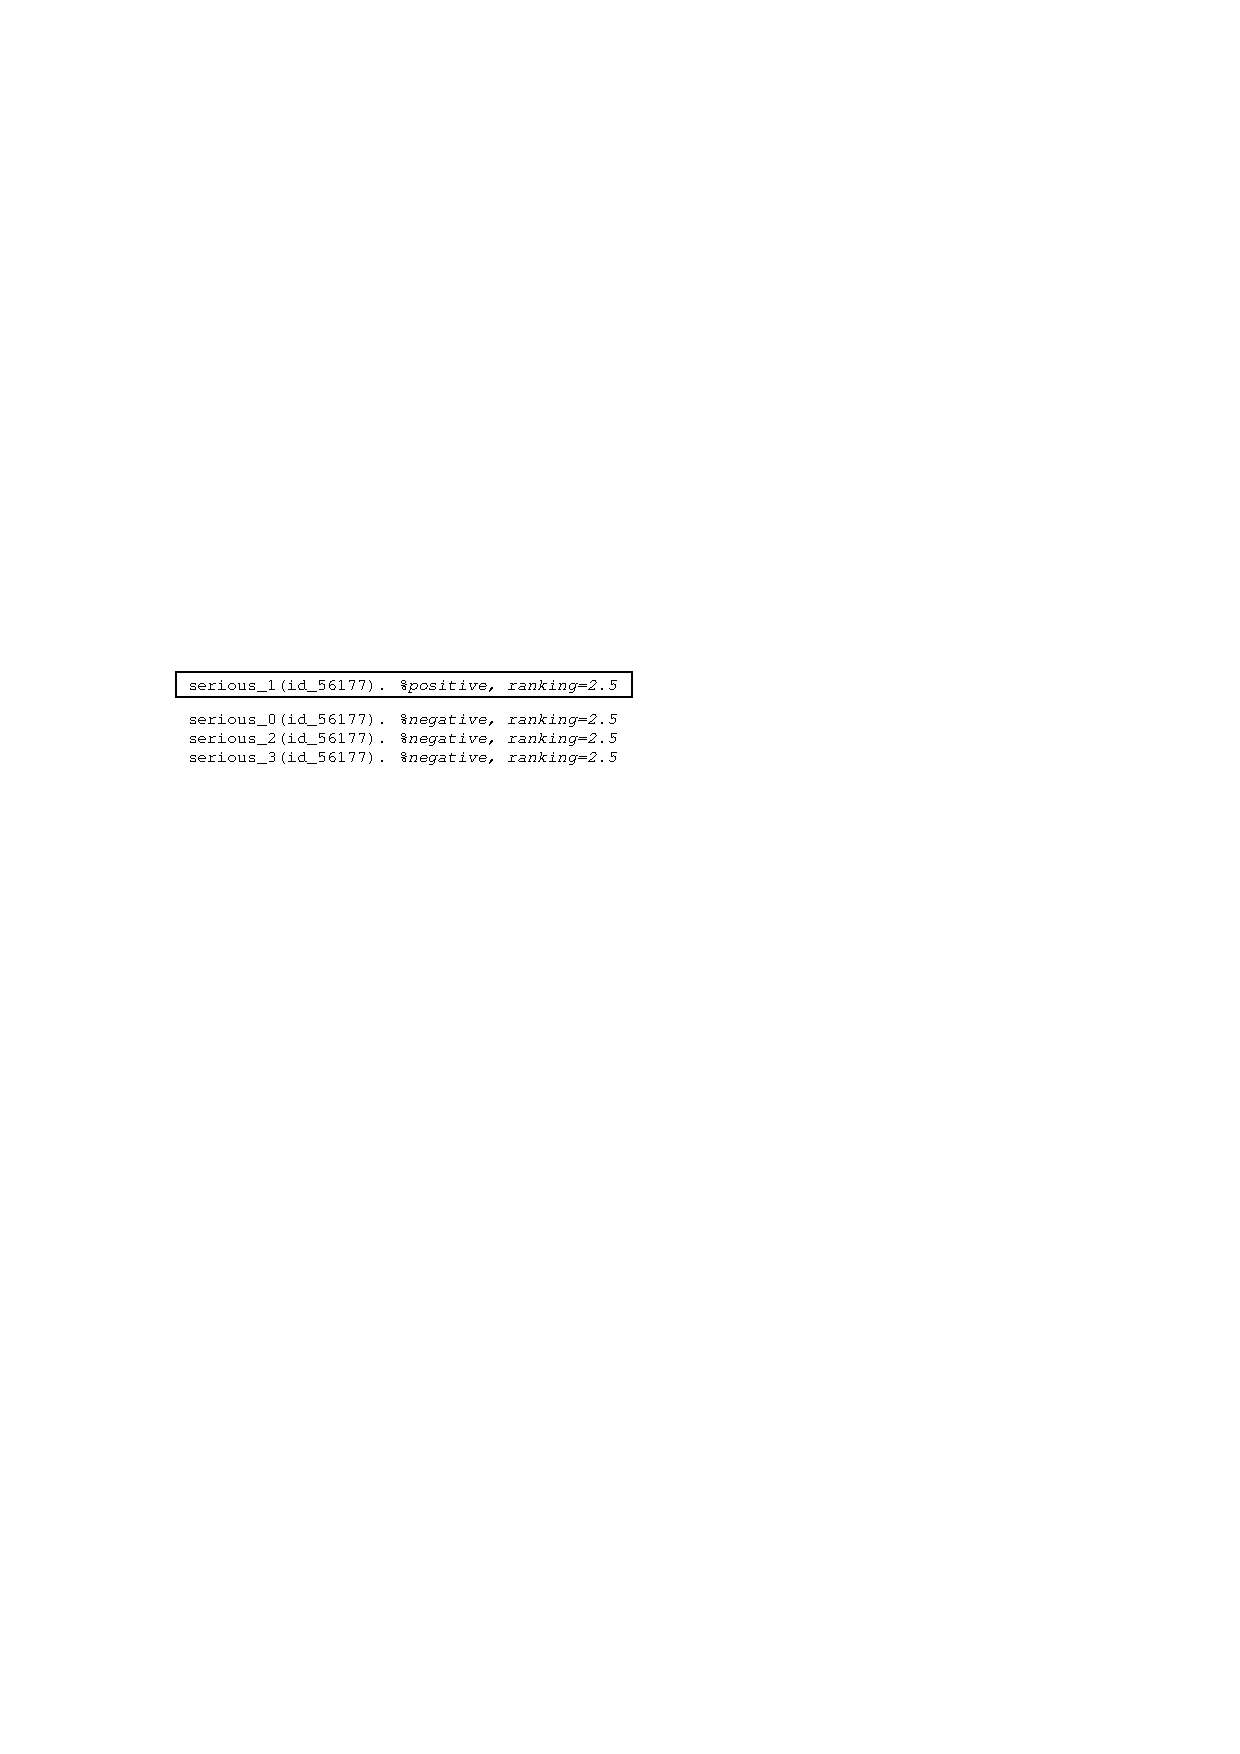
\includegraphics[width=.8\hsize]{img/examples_nonmonot}}
Monotonized learning examples\\
\centerline{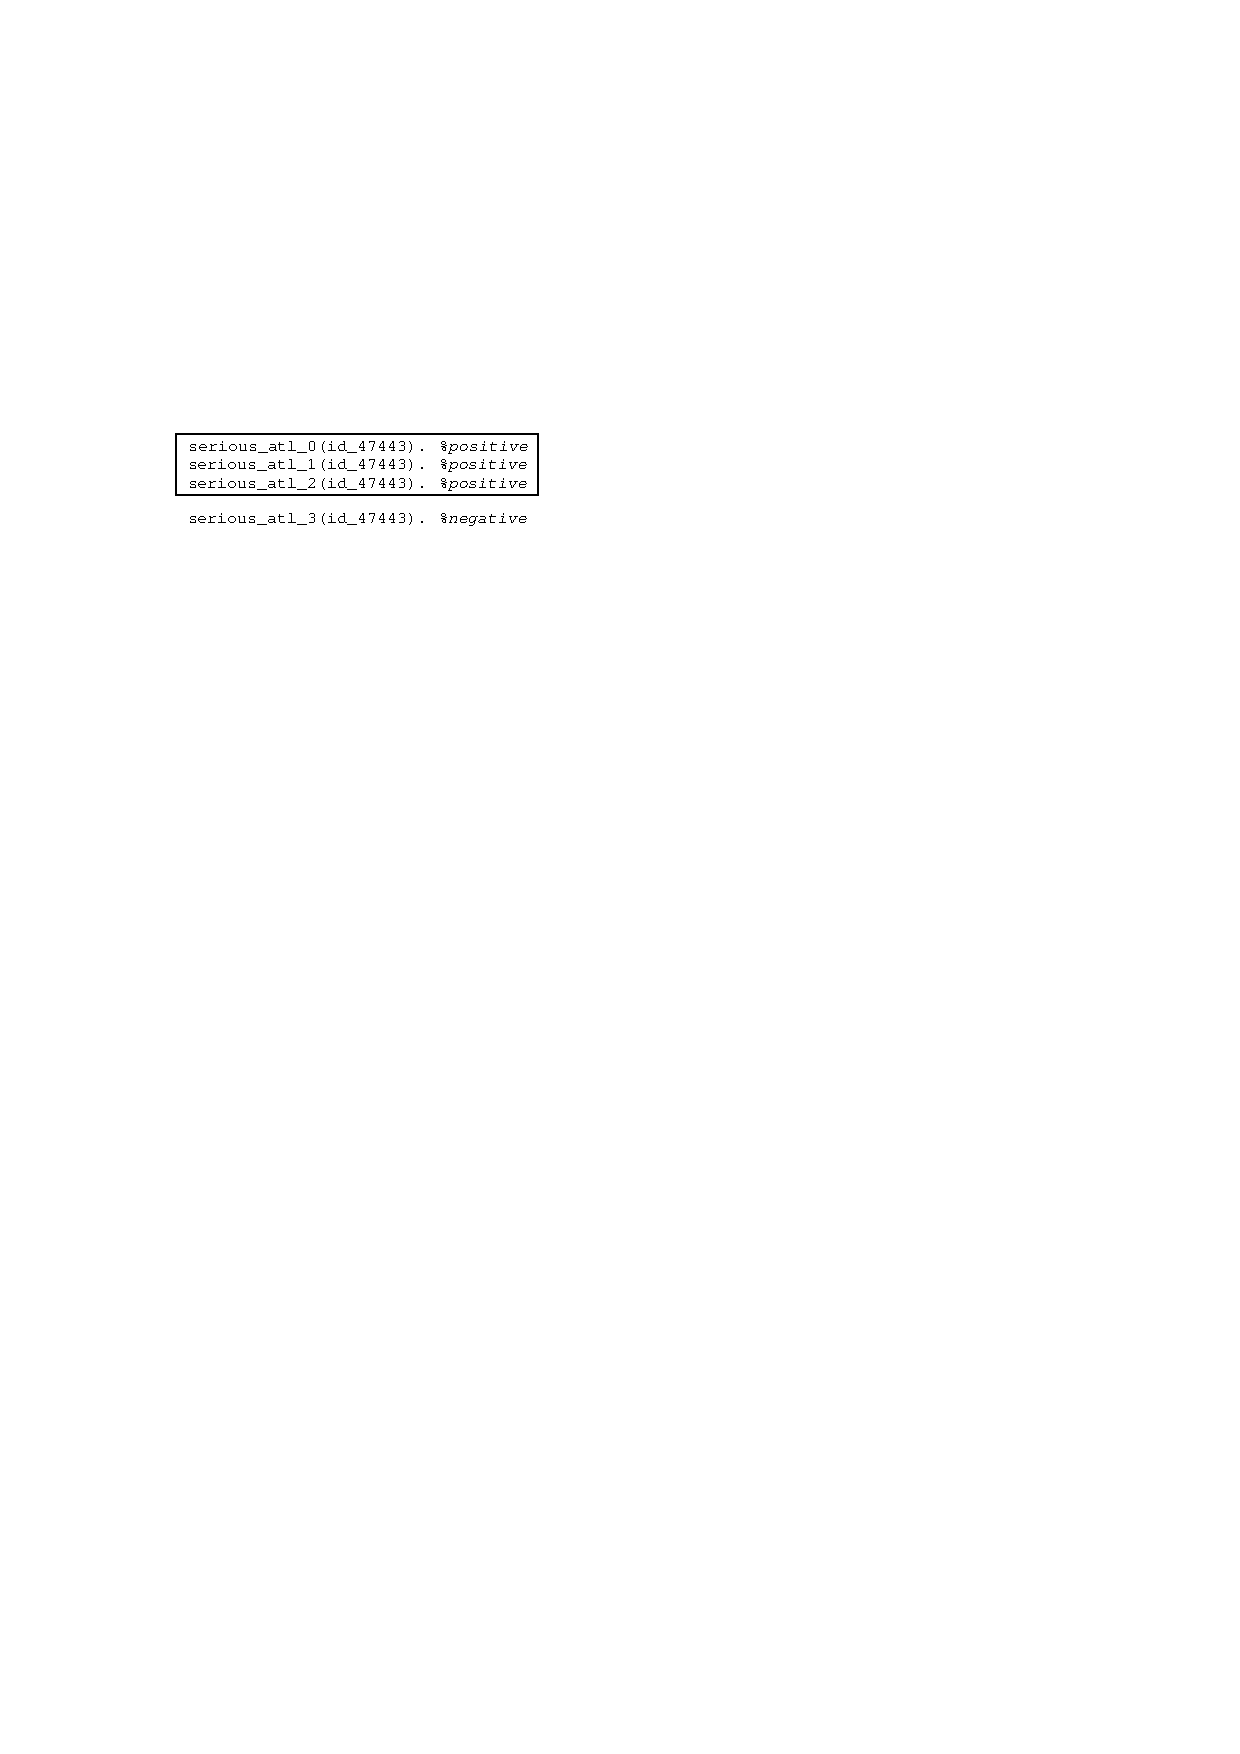
\includegraphics[width=.8\hsize]{img/examples_monot}}
\caption{Learning examples.}
\label{img:examples}
\end{figure}

\begin{figure}[b!]
damage $\rightarrow$ damage\_atl\\
\centerline{
\includegraphics[width=.8\hsize]{img/attribute_monotonisation}}
\caption{Monotonization of attributes.}
\label{img:attribute_monotonization}
\end{figure}


%%%%%%%%%%%%%%%%%%%%%%%%%%%%%%%%%%%%%%%%%%%%%%%%%%%%%%%%%%%%%%%%%%%%%%%%%%%%%%%%%%%%%%%%%%%%%%%%%
\section{The system prototype and our experiment}
%%%%%%%%%%%%%%%%%%%%%%%%%%%%%%%%%%%%%%%%%%%%%%%%%%%%%%%%%%%%%%%%%%%%%%%%%%%%%%%%%%%%%%%%%%%%%%%%%
The main experiment presented in this paper leads to the seriousness classification of an accident presented on a web report, %Our long term goal is extraction of semantic information from web reports. 
which is one of possible utilizations of the extracted semantic information. We use web reports of fire departments of several regions of the Czech Republic. These reports are written in Czech language and can be accessed through the web of General Directorate of the Fire and Rescue Service of the Czech Republic\footnote{\url{http://www.hzscr.cz}}. 
%These reports are rich in information, e.g. where and when an traffic accident occurred, which units helped, how much time it took them to show up on the place of accident, how many people were injured, killed etc.

For the present experiment we have selected a collection of 50 web reports. We have identified several features presented in these reports and manually extracted corresponding values. This will be described in more detail in section \ref{sec:features}. To each report we have also assigned a value of overall ranking of seriousness of presented accident, which is the target of the classification.

%There are two objectives to do. Fist is the web information extraction, a long path starting with web crawling and resulting with the extracted structured information. Second is the seriousness classification, which utilizes the extracted information. We have made much work on the first (see e.g. %\cite{biblio:DeVoLinguisticextraction2008,biblio:DeVoComputingaggregations2008, biblio:DeEcExperimentswith2008}), in this paper we will concentrate on the second.
%\cite{biblio:DeEcExperimentswith2008}), in this paper we will concentrate on the second.



%%%%%%%%%%%%%%%%%%%%%%%%%%%%%%%%%%%%%%%%%%%%%%%%%%%%%%%%%%%%%%%%%%%%%%%%%%%%%%%%%%%%%%%%%%%%%%%%%
%\subsection{Experiment description} \label{sec:experiment_desc}
%%%%%%%%%%%%%%%%%%%%%%%%%%%%%%%%%%%%%%%%%%%%%%%%%%%%%%%%%%%%%%%%%%%%%%%%%%%%%%%%%%%%%%%%%%%%%%%%%

For the seriousness classification we have used two inductive logic approaches -- Classical ILP and Fuzzy ILP (as described above). Technically the difference between the approaches consist in different setting of \emph{ILP task}. Both can be done with a classical ILP tool. We have used 
``\emph{A Learning Engine for Proposing Hypotheses}'' (Aleph  v5\footnote{\url{http://www.comlab.ox.ac.uk/activities/machinelearning/Aleph/}}), which seems very practical to us. It use quite effective method of \emph{inverse entailment} \cite{biblio:InverseEntailment} and keeps all handy features of Prolog system (supports YAP and SWI) in its background.

We have compared results of the two approaches (fuzzy and classical) and we could see that the fuzzy approach made better results than the classical one. See section \ref{sec:results} for details of the results.




%%%%%%%%%%%%%%%%%%%%%%%%%%%%%%%%%%%%%%%%%%%%%%%%%%%%%%%%%%%%%%%%%%%%%%%%%%%%%%%%%%%%%%%%%%%%%%%%%
\subsection{Features of accidents} \label{sec:features}
%%%%%%%%%%%%%%%%%%%%%%%%%%%%%%%%%%%%%%%%%%%%%%%%%%%%%%%%%%%%%%%%%%%%%%%%%%%%%%%%%%%%%%%%%%%%%%%%%



Figure \ref{img:attributes_description} summarizes all features (or attributes) that we have obtained from accident reports. Except the attribute \verb+type+ (type of an accident -- \verb+fire+, \verb+car_accident+ and \verb+other+) all the attributes are numerical and so monotonizable. In some cases value of some attribute is unknown. We have decided to make evidence of this and keep the values \verb+unknown+ in a knowledge base. Short explanation of each attribute follows.
\newline
\verb+size+ is a file size of text part of a report.\\
	\verb+damage+ is an amount (in CZK -- Czech Crowns) of summarized damage arisen during an accident.\\
	\verb+dur_minutes+ is time (minutes) taken to handle an accident.\\
	\verb+fatalities+ and \verb+injuries+ are numbers of fatalities (and injuries) taken by an accident.\\
	\verb+cars+ is number of cars damaged during an accident (especially during car accidents).\\
	\verb+professional_units+ and \verb+amateur_units+ are numbers of fireman units sent for an accident.\\
	\verb+pipes+ is number of  used fire pipes.\\
	\verb+lather+, \verb+aqualung+ and \verb+fan+ (ventilator) indicates weather these devices were used.


%%%%%%%%%%%%%%%%%%%%%%%%%%%%%%%%%%%%%%%%%%%%%%%%%%%%%%%%%%%%%%%%%%%%%%%%%%%%%%%%%%%%%%%%%%%%%%%%%
\subsection{Seriousness ranking} \label{sec:seriousness}
%%%%%%%%%%%%%%%%%%%%%%%%%%%%%%%%%%%%%%%%%%%%%%%%%%%%%%%%%%%%%%%%%%%%%%%%%%%%%%%%%%%%%%%%%%%%%%%%%


%\begin{figure}
%\centerline{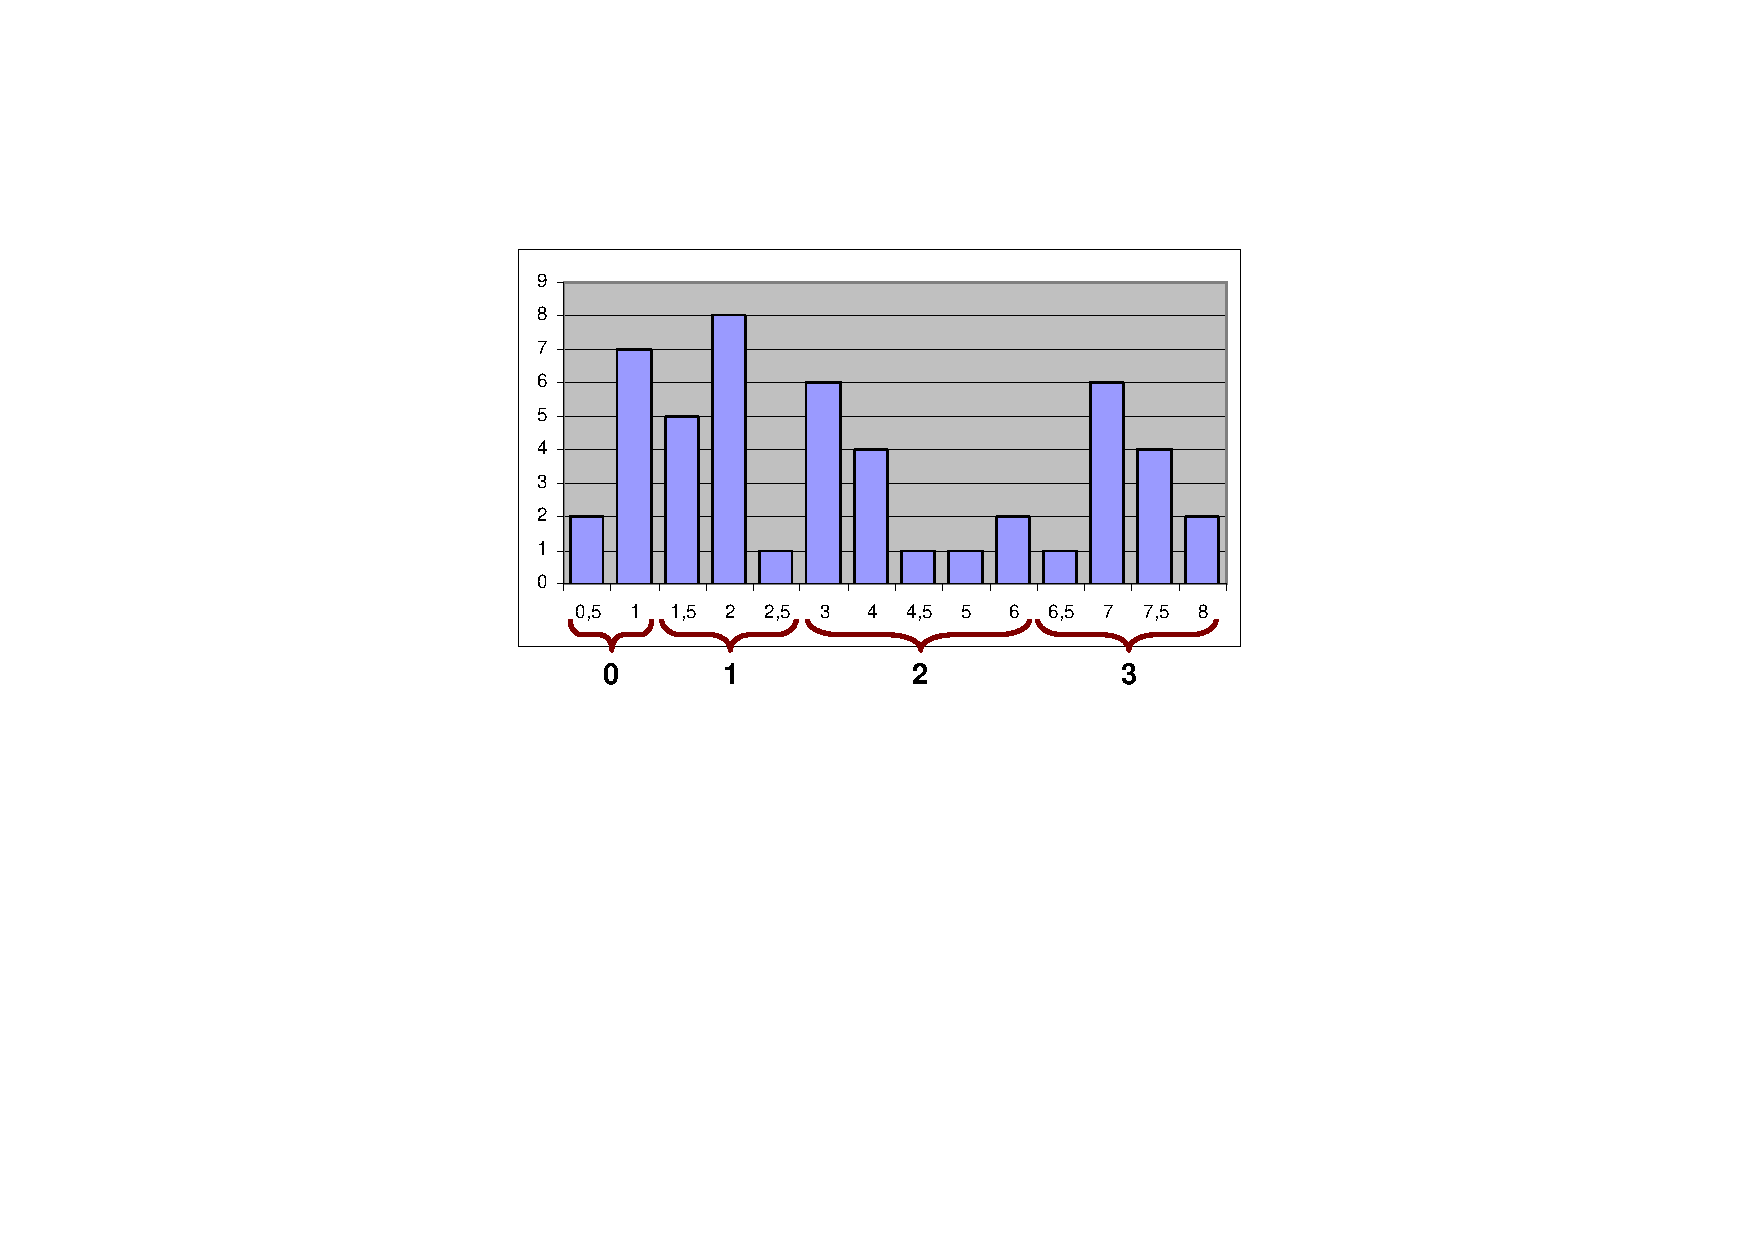
\includegraphics[width=\hsize]{img/ranking_histogram}}
%\caption{Frequencies of accident ranking.}
%\label{img:ranking_histogram}
%\end{figure}

Values of overall seriousness ranking attribute were stated from ``general impression'' from report's texts with respect to the particular attributes. %(Fig~\ref{img:attributes_description}). 
Values of seriousness ranking have evolved to 14 distinct values in range form 0.5 to 8. 
%Histogram with frequencies of all the values is on the Figure~\ref{img:ranking_histogram}.
We have divided the values into four approximately equipotent groups 
%(shown on the Fig.~\ref{img:ranking_histogram}) 
and learned logic rules for each group separately.


%%%%%%%%%%%%%%%%%%%%%%%%%%%%%%%%%%%%%%%%%%%%%%%%%%%%%%%%%%%%%%%%%%%%%%%%%%%%%%%%%%%%%%%%%%%%%%%%%
\subsection{Data transformation} \label{sec:data_transformation}
%%%%%%%%%%%%%%%%%%%%%%%%%%%%%%%%%%%%%%%%%%%%%%%%%%%%%%%%%%%%%%%%%%%%%%%%%%%%%%%%%%%%%%%%%%%%%%%%%

As already described in previous section, we have two possibilities to organize crisp ILP tasks, one with raw data and second with monotonized data. For this we have to translate extracted data. 

For the construction of the $E_t$ example set in our application we encode it in the predicate \texttt{serious\_t}, For the construction of the $E_{\ge t}$ example set in our application we encode it in the predicate \texttt{serious\_atl\_t}, see Fig~\ref{img:examples}.





%\begin{figure}
%\centerline{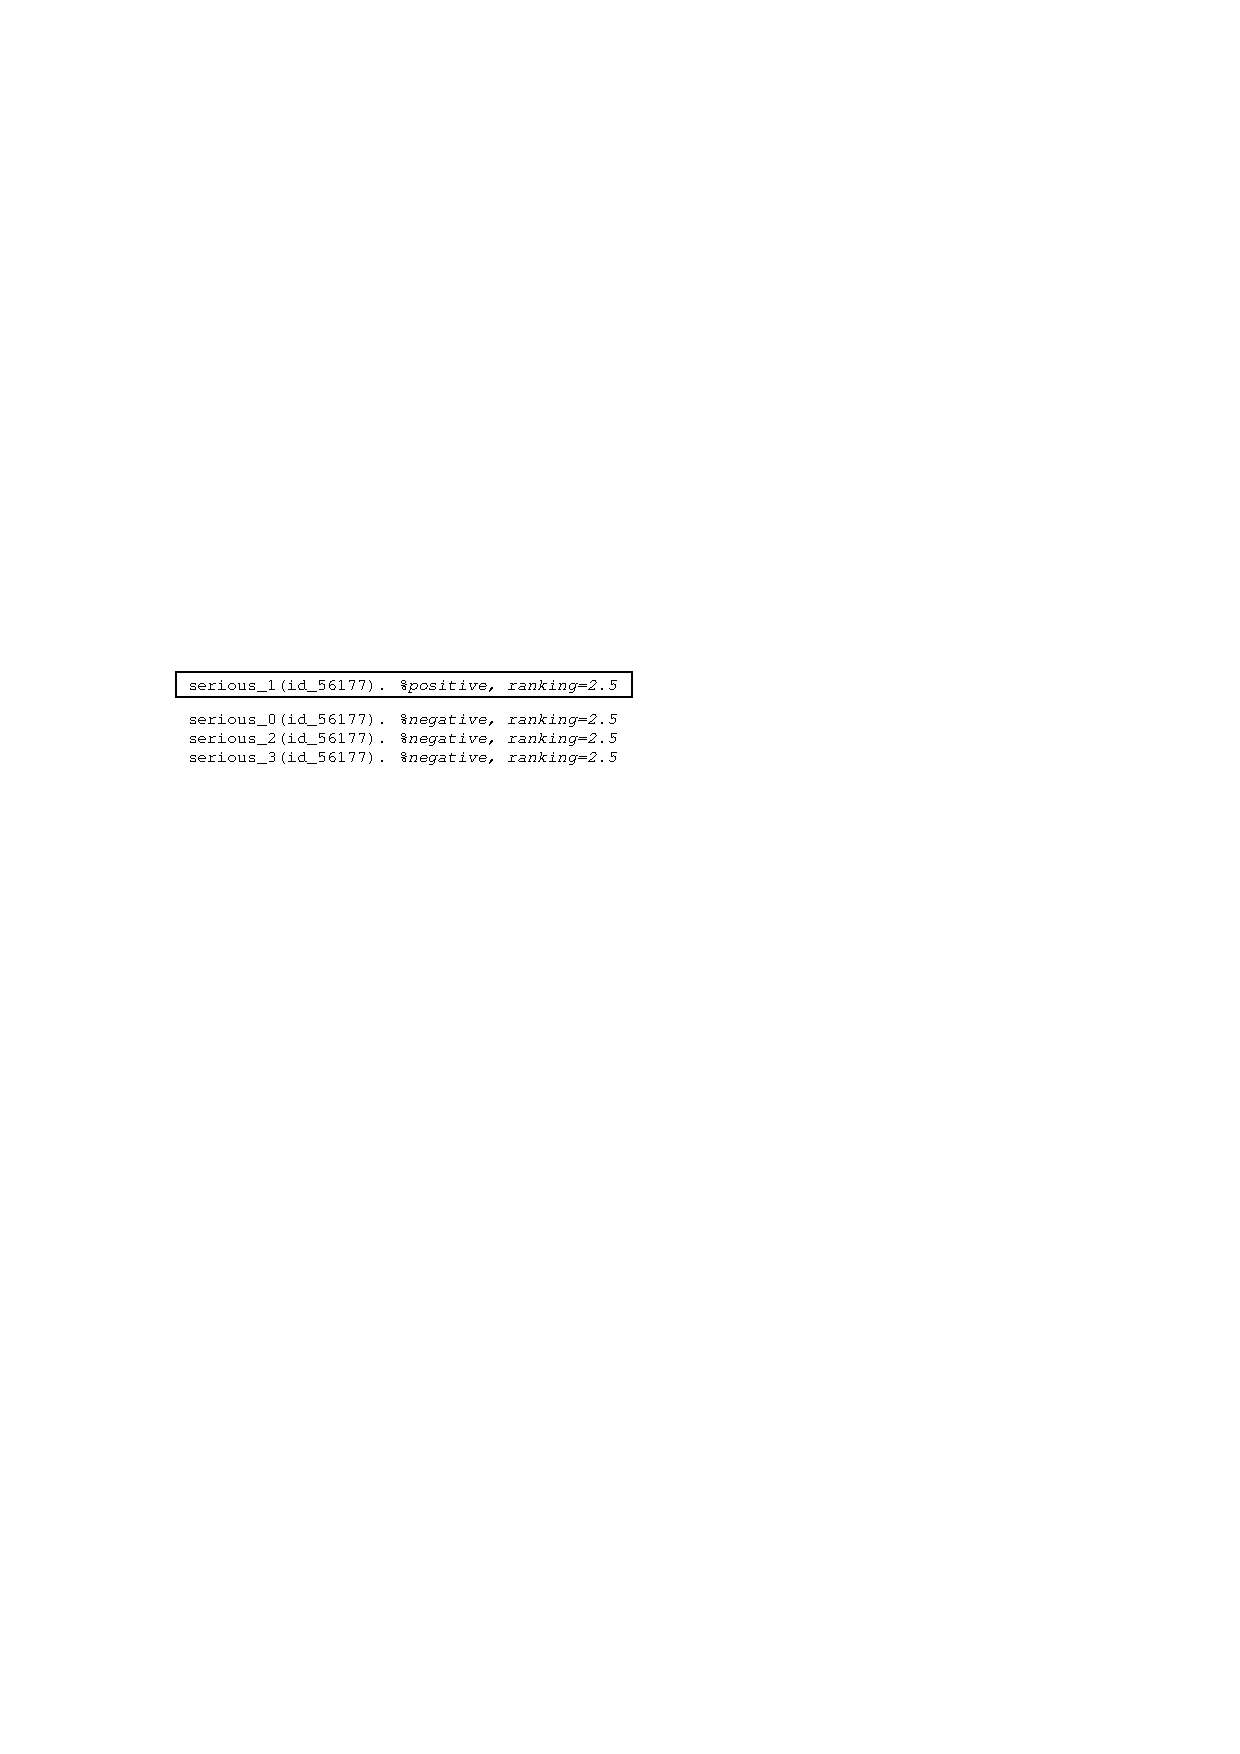
\includegraphics[width=.8\hsize]{img/examples_nonmonot}}
%\caption{Crisp learning examples.}
%\label{img:examples_nonmonot}
%\end{figure}
%
%\begin{figure}
%\centerline{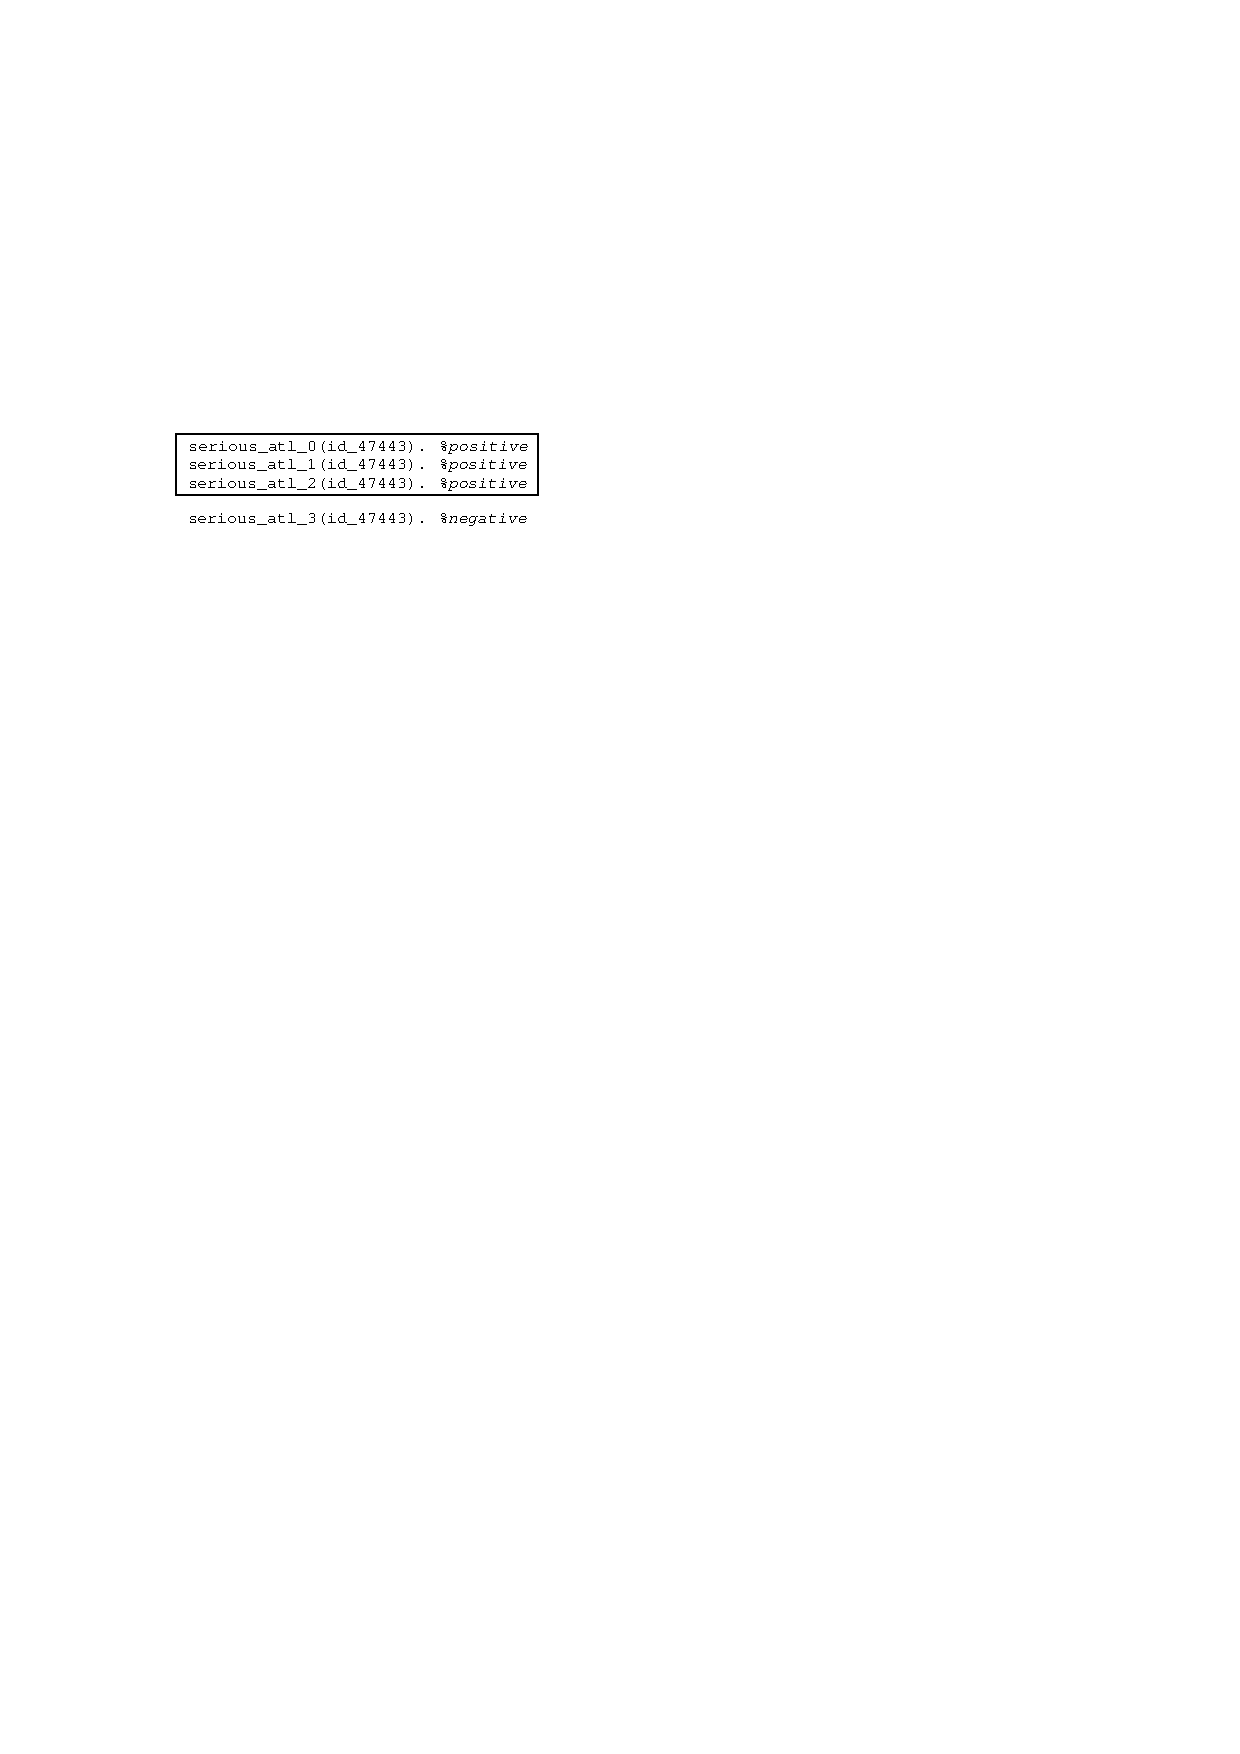
\includegraphics[width=.9\hsize]{img/examples_monot}}
%\caption{Monotonized learning examples.}
%\label{img:examples_monot}
%\end{figure}
%
For the construction of monotonized set of background knowledge $B^{mon}_T$ we use rules, here illustrated on predicates \texttt{damage} and \texttt{damage\_atl}, see Fig~\ref{img:attribute_monotonization}. Here, first rules deals with \texttt{unknown} values and the second constructs the translation.


\begin{figure}
\centerline{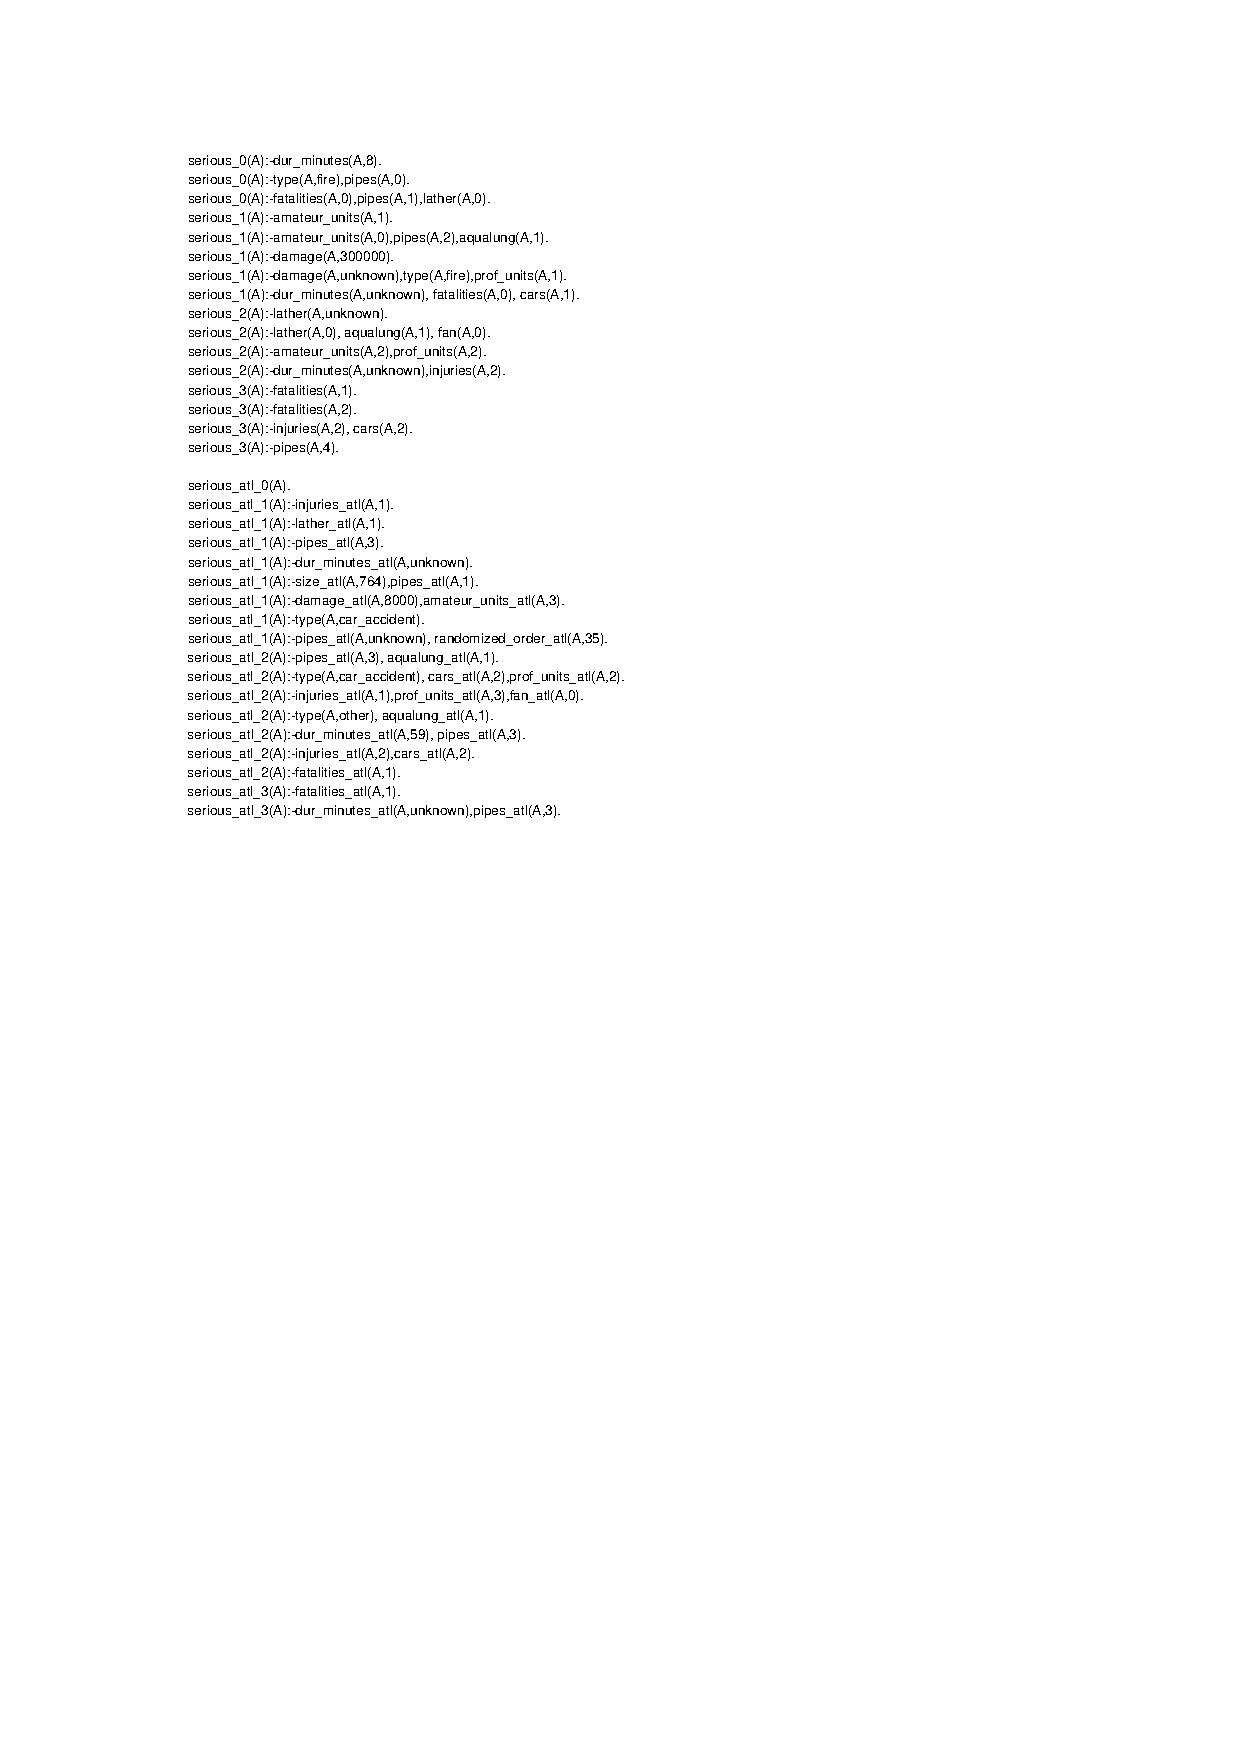
\includegraphics[width=\hsize,height=\hsize]{img/rules}}
\caption{Crisp \& monotonized hypothesis}
\label{img:rules}
\end{figure}

%\begin{figure}
%\centerline{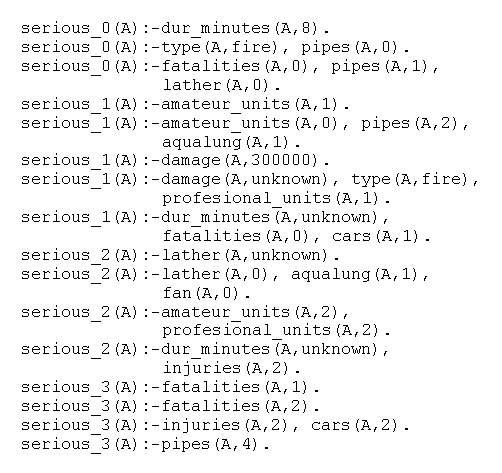
\includegraphics[width=\hsize]{img/rules_nonmonot}}
%\caption{Crisp hypothesis}
%\label{img:rules_nonmonot}
%\end{figure}
%
%\begin{figure}
%\centerline{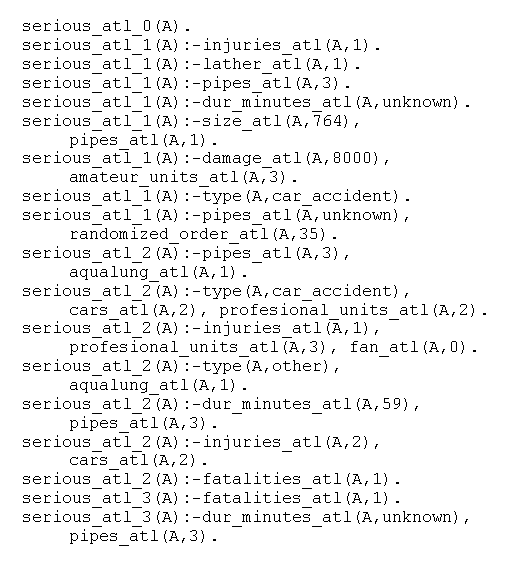
\includegraphics[width=\hsize]{img/rules_monot}}
%\caption{Monotonized hypothesis}
%\label{img:rules_monot}
%\end{figure}


%%%%%%%%%%%%%%%%%%%%%%%%%%%%%%%%%%%%%%%%%%%%%%%%%%%%%%%%%%%%%%%%%%%%%%%%%%%%%%%%%%%%%%%%%%%%%%%%%
\section{Results} \label{sec:results}
%%%%%%%%%%%%%%%%%%%%%%%%%%%%%%%%%%%%%%%%%%%%%%%%%%%%%%%%%%%%%%%%%%%%%%%%%%%%%%%%%%%%%%%%%%%%%%%%%



The Fig~\ref{img:rules} summarizes sets of obtained rules from two experiments: 
\\(1) experiments with $E_t$ and $B^{raw}_{T}$
\\(2) experiments with $E_{\ge t}, {B}^{mon}_T$.

%Experiments with $E_t$ and $B^{raw}_{T}$ %Results of experiments with $E_t$ and $B^{raw}_{T}$ 
%gave following rule set, see Fig~\ref{img:rules_nonmonot}.

Evaluation of learning is depicted in the Fig~\ref{img:evaluation}.

%\subsection{Experiments $E_{\ge t}, {B}^{mon}_T$}



%Evaluation of learning is depicted in the green area of Fig~\ref{img:evaluation}.

%\subsection{Evaluation and comparison }

We wanted to compare raw and monotonized learning tasks. As they run on different example sets we had translate results of one learning (rules with head \texttt{serious\_t}) to results of second learning (rules with head \texttt{serious\_atl\_t}). Logic programming translation rules are depicted on Fig~\ref{img:monot2nomon_and_invert}.


\begin{figure}
crisp $\rightarrow$ monotone\\
\centerline{
\includegraphics[width=.8\hsize]{img/nomon2monot}}

monotone $\rightarrow$ crisp\\
\centerline{
\includegraphics[width=.8\hsize]{img/monot2nomon}}
\caption{Conversion of results}
\label{img:monot2nomon_and_invert}
\end{figure}

%\begin{figure}
%\centerline{
\includegraphics[width=.8\hsize]{img/nomon2monot}}
%\caption{Results conv.: crisp $\rightarrow$ monotone.}
%\label{img:nomon2monot}
%\end{figure}
%
%
%
%
%\begin{figure}
%\centerline{
\includegraphics[width=.8\hsize]{img/monot2nomon}}
%\caption{Results conv.: monotone $\rightarrow$ crisp.}
%\label{img:monot2nomon}
%\end{figure}

Then the comparison of both learnings is possible, see white areas of Fig~\ref{img:evaluation}.



\begin{figure}
\centerline{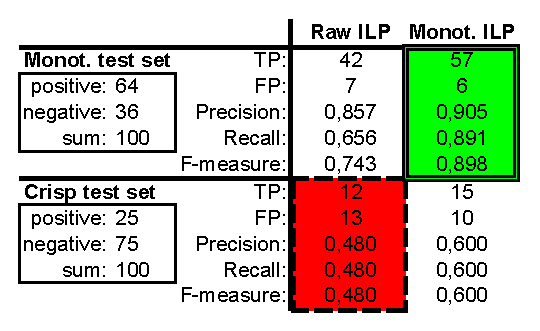
\includegraphics[width=0.8\hsize]{img/Evaluation}}
\caption{Evaluation results}
\label{img:evaluation}
\end{figure}

%%%%%%%%%%%%%%%%%%%%%%%%%%%%%%%%%%%%%%%%%%%%%%%%%%%%%%%%%%%%%%%%%%%%%%%%%%%%%%%%%%%%%%%%%%%%%%%%%
\section{Conclusion}
%%%%%%%%%%%%%%%%%%%%%%%%%%%%%%%%%%%%%%%%%%%%%%%%%%%%%%%%%%%%%%%%%%%%%%%%%%%%%%%%%%%%%%%%%%%%%%%%%
In this paper we have presented a fuzzy system which provides a fuzzy classification of textual web reports. Our approach was based on usage of third party linguistic analyzer, our previous work on web information extraction and fuzzy inductive logic programming. Main contributions are formal models and prototype implementation of the system and evaluation experiments with the Fuzzy ILP classification method. 

Experiments have shown better results of fuzzy approach. We see the difference in the fact that monotonization leads to the extension of the learning domain.

%Use of ILP was necessary for multirelational character of extracted data (relational representation of XML like form of PDT2.0 tectogramatical trees). 
%
%System need user assistance: of a skilled user in annotating data for extraction and an unskilled user for classification of a small training example set. This feature is especially important, because in Internet application, we cannot expect an unskilled user to classify a big number of examples 

\section*{Acknowledgment}
This work was partially supported by Czech projects IS-1ET100300517, GACR-201/09/H057 and MSM-0021620838.



\bibliographystyle{latex8}
\bibliography{DedekVojtas_WI_FuzzyILP}


\end{document}



%%% Local Variables: 
%%% mode: latex
%%% TeX-master: t
%%% End: 
